\chapter{Related Work}
\label{chapter:related}

%\begin{chapabstract}
%      Deep Learning is now the major method to learn unstructured data such as images. Computer
%      Vision used for a long time handcrafted convolution kernels, but nowadays, they are learned:
%      each value of the kernel is a neuron. This kind of network, called \acf{CNN}, showed
%      impressive performance in a wide variety of tasks. However, they still suffer from the plague
%      of forgetting when learning a moving distribution as new samples, from new sources or new
%      classes appear. Continual Learning aims to solve this challenge using multiple
%      approaches, including rehearsal and behavior constraints.
%\end{chapabstract}

%\minitoc
\chapterwithfigures{\nameref*{chapter:related}}
\chapterwithtables{\nameref*{chapter:related}}

\ifthenelse{\boolean{skipRelated}}{\endinput}{}


In this chapter, we detail the related work needed to read this thesis. We first briefly
explain the learning procedure in \acf{DL} and how the data are structured. Then, we describe the main
\ac{DL} applications and architectures in \acf{CV}. Finally, we introduce the main topic of this thesis
---Continual Learning--- and showcase the challenges, benchmarks, and methods of this domain. The
notations introduced in this chapter and through the thesis are listed in the
\hyperref[chap:notations]{Notations} section.

\section{Neural Network Learning}

Neural Networks are based on the statistical learning theory \citep{vapnik1999statstheory}. In the
\textit{supervised setting}, the goal of a neural network is to learn the best mapping function $f :
      \mathcal{X} \rightarrow \mathcal{Y}$ between an input space $\mathcal{X}$ and an output space
$\mathcal{Y}$.  We consider a \textit{loss} function $\mcL : \mathcal{Y} \times \mathcal{Y}
      \rightarrow \mathbb{R}^+$ that measures the disagreement between a ground-truth label $y$ and the
network's prediction $\hat{\vy} = f(\vx)$. In the context of image classification, $\vx$ is the
image pixels, $y$ is the \textit{class} label of the object present in the image, and $\hat{\vy}$ is
a vector of probabilities, with one probability per class the model has to predict. The class with
the highest predicted probability/confidence is chosen as the prediction. Given a \textit{training
      dataset} $\mathbb{D} = \{(\vx_1, y_1), ..., (\vx_N, y_N)\}$, training a neural network consists in
finding the set of parameters $\theta_*$ which minimizes the loss function:
%
\begin{equation}
      \theta_* = \operatorname{argmin}_{\theta} \left \{ \frac{1}{|\mathbb{D}|}\sum_{(\vx,y)\in \mathbb{D}} \mcL(f_\theta(\vx), y)\right \}\,.
      \label{eq:intro_optim}
\end{equation}
%
However, the optimal set of parameters $\theta_*$ minimizing the loss on the training set, can fail
to predict the correct label on the testing set. Therefore, to avoid this \textit{overfitting}
phenomenon, regularization functions that limit the parameters space are used as additional
constraints in addition to the classification loss $\mcL$.

In practice, the function $f_\theta$ learned by a neural network is composed of a succession of
linear transformations and non-linear \textit{activation} functions. For example, a simple neural
network, called \ac{MLP}, here with two layers, could be defined as:
%
\begin{equation}
      \hat{\vy} = f_\theta(\vx) = \operatorname{softmax}(\vW_o \sigma(\vW_h \vx + \vb_h) + \vb_o))\,,
      \label{eq:intro_mlp}
\end{equation}
%
\noindent with $\vW_h \in \mathbb{R}^{H \times D}$, $\vb_h \in \mathbb{R}^{H}$, $\vW_o \in
      \mathbb{R}^{C \times H}$, $\vb_o \in \mathbb{R}^{C}$ being the parameters $\theta$ of the
network. $\sigma$ is a hidden non-linear activation, often a \ac{ReLU}
($\operatorname{ReLU(x)} = \text{max}(0, x)$), and $\hat{y} = \operatorname{softmax}(\tilde{\vy}) =
      \nicefrac{e^{\tilde{\vy}}}{\sum_{i} e^{\tilde{\vy}_i}}$ is the final non-linear activation.

Likewise, in practice for image classification, the loss is often the categorical cross-entropy:
%
\begin{equation}
      \mcL(\hat{\vy}, \vy) = -\sum_c y_c \log \hat{y}_c\,,
      \label{eq:intro_ce}
\end{equation}
%
\noindent with $\vy$ a one-hot vector of the labels. Finally, to optimize the parameters of the neural
network (such as \autoref{eq:intro_optim}), we often use the mini-batch \ac{SGD} algorithm or a variation thereof:

\begin{algorithm}
      \begin{algorithmic}[1]
            \Statex \textbf{input:} a dataset $\mathbb{D}$ with pairs of $(\vx_i, \vy_i)$
            \Statex \textbf{input:} a loss function $\mcL$
            \Statex \textbf{input:} a model function $f_\theta$ with $\theta$ the learned parameters
            \Statex \textbf{input:} a learning rate $\eta$ and a batch size $b$
            \Statex

            \While{stopping criterion not satisfied}
            \State $(\vx, \vy)$ $\gets$ sample mini-batch of size $b$ from $\mathbb{D}$
            \State Forward pass: $\hat{\vy}$ $\gets$ $f_\theta(\vx)$
            \State Compute loss: $\mcL$ $\gets$ $\mcL(\hat{\vy}, \vy)$
            \State Compute the gradients: $\delta$ $\gets$ $\nabla_\theta \mcL$
            \State Update all parameters: $\theta$ $\gets$ $\theta - \eta \delta$
            \EndWhile
      \end{algorithmic}
      \caption{Procedure to optimize a neural network with gradient descent.}
      \label{algo:intro_sgd}
\end{algorithm}

The learning rate $\eta$ controls the step size when updating the parameters in the direction of the
gradient. The batch size $b$ defines the number of images seen during one update. The
\textit{backpropagation} algorithm \citep{rumelhart1986backprop} computes the gradients and the
update of the parameters. In the case of image classification and segmentation, the main topics
explored in this thesis, we discern the \textit{feature extractor} from the \textit{classifier} in
the neural network. The former transforms the input space so that the latter linearly discriminates
classes. From now on, the feature extractor will be denoted by $f$, and the classifier by $g$ (see
the \hyperref[chap:notations]{notations}). The model is then $g \circ f$.

The neural network in \autoref{eq:intro_mlp} can be defined as \textit{shallow} with only one hidden
layer. By extension, an important success of later neural networks came with training \textit{deep}
neural network with multiple hidden layers. More generally in this thesis, we will refer to them as
\acf{DL} models. The majority of \ac{DL} models, in \acf{CV}, in \acf{NLP}, or even in Audio are
based on the same structure (linear transformations and non-linear activations) and are trained with
a form of gradient descent.

\section{Deep Architectures for Computer Vision}
\label{sec:related_cv}

A common type of architectures for computer vision is the \acf{ConvNet}. First defined by
\citet{fukushima1980neocognitron} and then trained with backpropagation by \citet{lecun1999lenet},
it is a neural network architecture whose linear operators are \textit{convolutions}. While
handcrafted convolutions \citep{lowe1999sift} rely on well-defined features, a \ac{ConvNet} learns
the convolution kernels to detect more complex patterns required to minimize the classification
loss. In 2012, thanks to a large dataset and more efficient code working on \acp{GPU} allowing
training larger networks, \citet{krizhevsky2012alexnet} won the ILSVC competition
\citep{russakovsky2015imagenet_ilsvrc} where they had to classify a large dataset ---ImageNet---
made of 1.28M training images and 1000 classes. From that point forward, multiple improvements were
made to \acp{ConvNet} \citep{ioffe2015batchnorm,he2016resnet} and these methods have been applied
not only to classification but also object detection \citep{ren20fasterrcnn}, semantic segmentation
\citep{chen2018deeplab}, visual question answering \citep{antol2015vqa,benyounes2017mutan}, image
generation \citep{goodfellow2014gan}, image editing \citep{grechka2021magecally,couairon2022flexit},
\etc.

Most \acp{ConvNet} follow a similar structure with blocks of convolutions and pooling. Often, the
final spatial features are flattened by \ac{GAP} and fed to a linear classifier
predicting the classes probabilities. \autoref{fig:related_cnn} illustrates this general architecture.

\begin{figure}[tb]
      \begin{center}
            \includegraphics[width=0.8\linewidth]{images/related/cnn.pdf}
      \end{center}
      \caption{\textbf{A Convolutional Neural Networks} extracts more complex patterns through its
            succession of convolutions. \textcolor{Goldenrod}{\textbf{Yellow}} blocks are
            convolutions, \textcolor{BurntOrange}{\textbf{orange}} blocks are poolings, and the
            unique \textcolor{ForestGreen}{\textbf{green}} block is the classifier. Given an image,
            the \ac{ConvNet} can assign to each possible class a probability, all summing to 1. The
            detected shapes grow in complexity with the depth of the network, from crude edges and
            textures, to objects. Detected patterns taken from \citet{olah2017feature}.}
      \label{fig:related_cnn}
\end{figure}

\paragraph{Architectures:}The 2010's decade saw major improvements to \acp{ConvNet}, both in their
architecture and in their training procedure. \citet{srivastava2015highwaynet} and
\citet{he2016resnet} propose residual connections between blocks likewise: $\vy = \vx +
      \sigma(\operatorname{Conv}(\vx))$. By reducing the \textit{vanishing gradient} problem
\citep{hochreiter2001vanishinggrad}, it allows training deeper networks without accuracy
degradation. This type of connection is now quasi-ubiquitous in all \ac{DL} based architectures.
Other architecture changes include using convolutions of different kernel sizes in parallel as in
Inception \citep{szegedy2015inception}, enabling a multi-scales view of the features. These
architectures are depicted in \autoref{fig:related_resnet_inception}.

\begin{figure}[tb]
      \begin{center}
            \includegraphics[width=\linewidth]{images/related/resnet_inception.pdf}
      \end{center}
      \caption{\textbf{Different ConvNet architectures:} \textbf{(a)} illustrates a ResNet-like
            architecture where there are residual connections between blocks. Used by the vast
            majority of modern architectures, these connections reduce the vanishing gradient problem
            and thus enabling the training of deeper networks. \textbf{(b)} showcases an Inception-like
            architecture where at the same level convolutions with different kernel sizes are used.
            Each detects patterns of different scales.}
      \label{fig:related_resnet_inception}
\end{figure}

\paragraph{Regularizations:} While the architecture design has an impact on the model performance,
the training procedure has been shown to be essential in order to reach state-of-the-art results
\citep{wightman2019resnetstrikesback}. Modern procedures include improvement of \ac{SGD} with an
adaptive learning rate per layer such as Adam \citep{kingma2014adam}, an improved learning rate
scheduling, stronger data augmentations
\citep{muller2021trivialaugment,hingyi2018mixup,zhong2017erasing}, and regularizations such as
Dropout \citep{gal2016dropout} and stochastic depth \citep{gao2016stochasticdepth}.

\paragraph{Transformers:} While convolution-based neural networks dominated \acf{CV} in the 2010's
decade, in the last few years, the transformer architecture gained interest: it was originally
designed for machine translation in \ac{NLP} \citep{vaswani2017transformer} with an encoder/decoder
structure and a \textit{self-attention} block between the words embeddings of a sentence. Each word is
embedded into a high-dimensional vector named a ``\textit{token}''. The self-attention operation of a
transformer has a quadratic complexity \wrt the number of tokens: in \ac{NLP}, it is manageable
given a small sentence. However, when applying a transformer on images and considering each pixel
as a token, the complexity is too important. \citet{dosovitskiy2020vit}, based on the encoder
structure of BERT \citep{devlin2018bert}, propose instead to consider a patch of pixels as a token,
reducing significantly the number of tokens.

\begin{figure}[tb]
      \begin{center}
            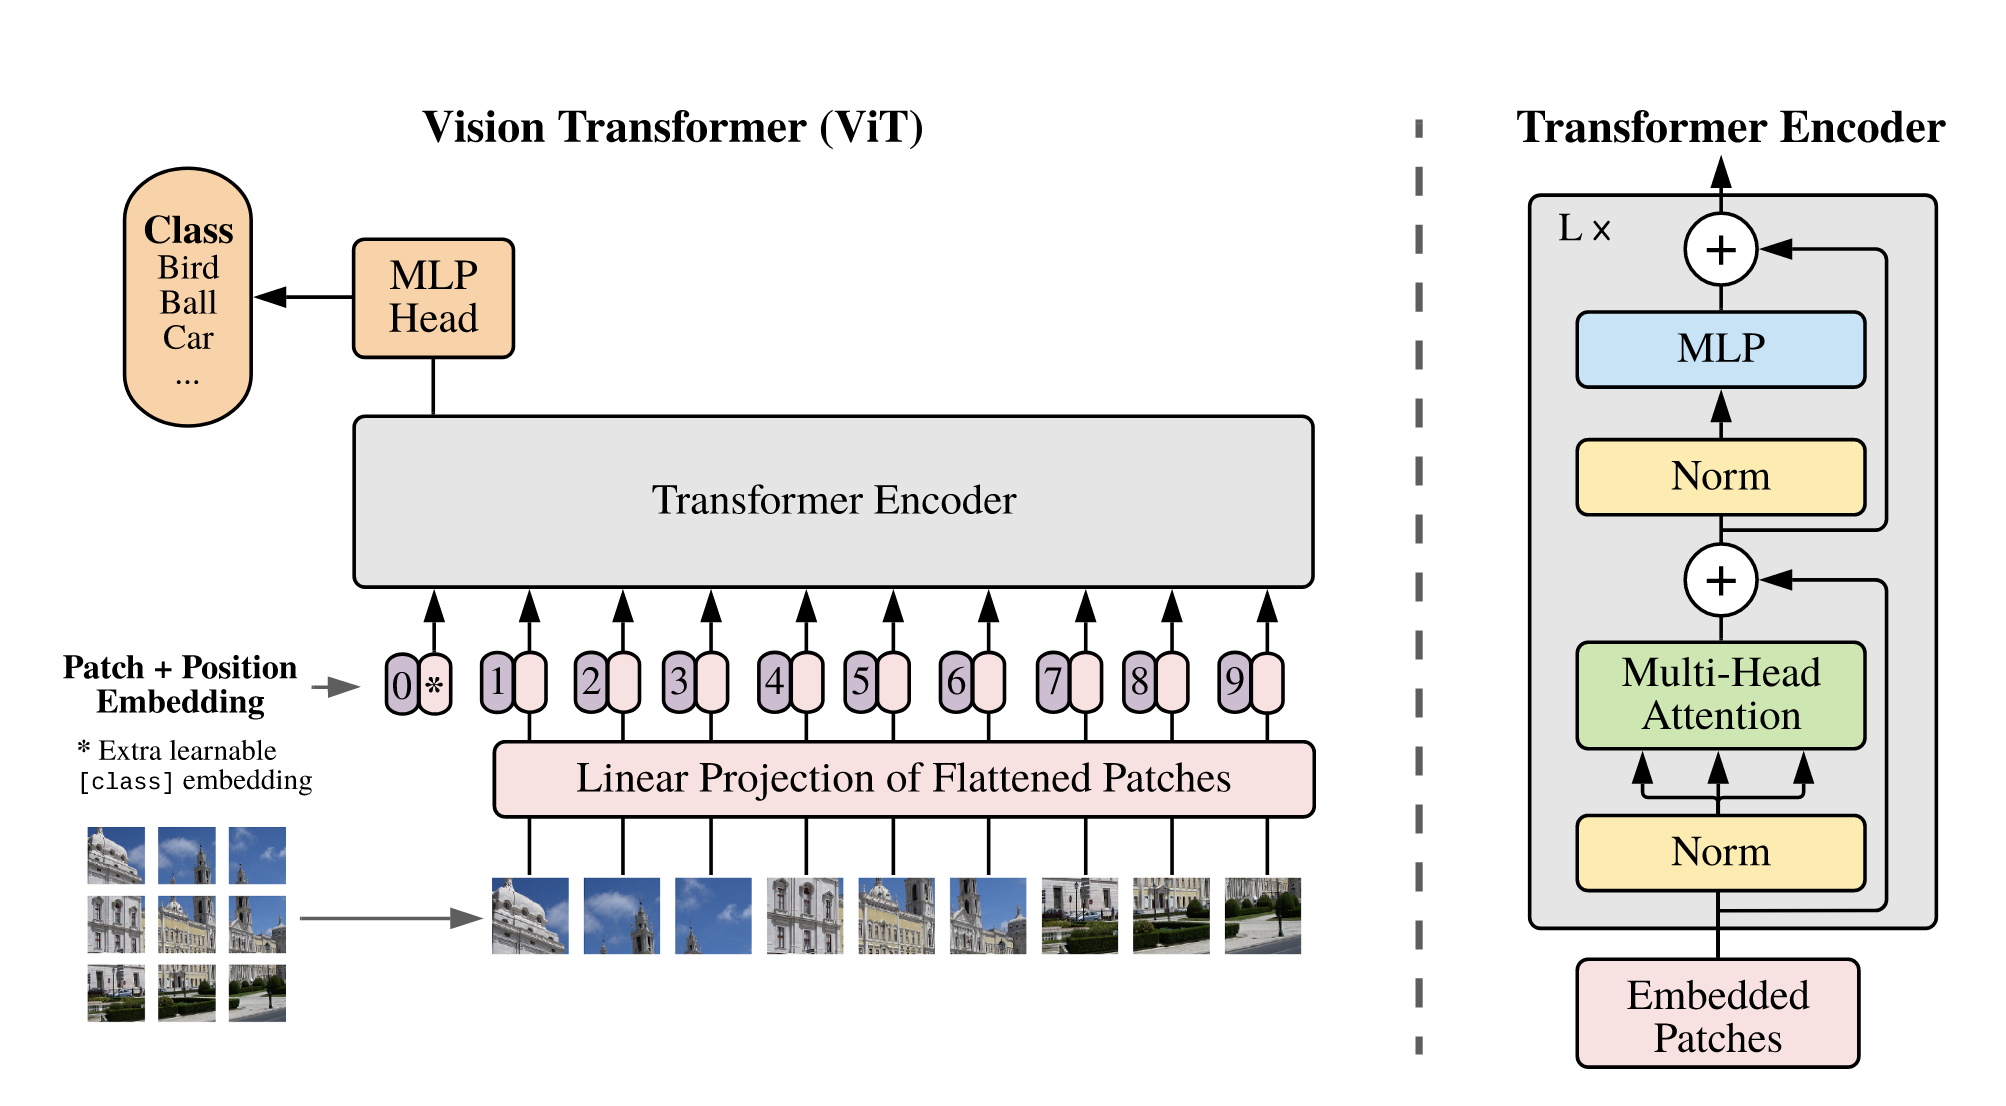
\includegraphics[width=\linewidth]{images/related/vit.png}
      \end{center}
      \caption{\textbf{The Vision Transformer (ViT):} the image is cropped without overlap and
            projected using a convolution whose stride equals the kernel size. A learned ``class
            token`` is concatenated to the resulting patches, which are then summed with a position
            embedding. The encoder is made of multiple transformer blocks. Each block is made of two
            (Layer) Norm layers, a MLP with a single hidden layer, and the Multi-Head Attention
            block. Finally, only the special ``class token'' is used at the end, and fed to a
            classifier (here denoted as the ``MLP Head''). Image from \citet{dosovitskiy2020vit}.}
      \label{fig:related_vit}
\end{figure}

This architecture is illustrated in \autoref{fig:related_vit}: we concatenate a special learned
token, called ``\textit{class token}'', to the patch tokens. Moreover, we also sum these tokens with
a position embedding to facilitate learning tokens position. Then, successive
transformer blocks process all the tokens. Each block is made of LayerNorms \citep{ba2016layernorm},
a self-attention block, a \ac{MLP}, and residual connections. Thus, the self-attention block is:
%
\begin{equation}
      \begin{aligned}
            Q & =W_{q} \vx\,,                                                       \\
            K & =W_{k} \vx\,,                                                       \\
            V & =W_{v} \vx\,,                                                       \\
            A & =\operatorname{Softmax}\left(Q \cdot K^{T} / \sqrt{D / h}\right)\,, \\
            O & = W_{o} A V+b_{o}\,,
      \end{aligned}
      \label{eq:related_sa}
\end{equation}
%
\noindent $\vx$ are the $N$ patch tokens and the class token, of shape $(N, D)$, $D$ being the
embedding dimension. The patch tokens are linearly transformed three times in parallel into a
\textbf{Q}uery, \textbf{K}ey, and \textbf{V}alue. An attention matrix $A$ of shape $(N, N)$ is
computed from the query $Q$ and the key $K$. Its $i^{\text{th}}$ row contains the similarity between
the $i^{\text{th}}$ token with all other tokens. Finally, the multiplication between the attention
matrix and the value matrix $V$ averages all tokens according to their similarities. To extend the
self-attention to its multi-heads variation (\ac{MHSA}), we use several Query/Key/Value
transformations, each used in a self-attention on a fraction of the embedding dimension.

ViT \citep{dosovitskiy2020vit} is the seminal paper on vision transformer. However, its training was
difficult and needed a large --- and private --- dataset called JFT300M. Later works, including DeiT
\citep{touvron2021deit} proposed an efficient optimization procedure enabling the training of
transformers on smaller datasets such as ImageNet \citep{russakovsky2015imagenet_ilsvrc}. Finally,
multiple works improved also the architecture itself, including CaiT \citep{touvron2021cait}, ConViT
\citep{dascoli2021convit}, and Swin \citep{liu2021swin}. Notably, PerceiverIO
\citep{jaegle2021perceiverio} proposed a general architecture whose output is adapted to different
modalities using specific learned tokens, and whose computation is reduced using a small number of
latent tokens.

\section{Continual Learning}
\label{sec:related_continual}

Usually, when training a \ac{ConvNet}, we assume the dataset is immutable and \textit{i.i.d.}: no new
images nor new classes will be learned. The knowledge acquired on one dataset \textit{A} can be
\textit{transferred} to another dataset \textit{B} with different classes using \textbf{transfer learning}
\citep{razavian2014transferlearning}. Then, the new model may be efficient on
the classes of dataset \textit{B} but cannot predict anymore the classes of dataset \textit{A}.

\textbf{Continual Learning} aims to learn a continually changing dataset without forgetting the
previous knowledge. The distribution of the dataset continually changes: \eg at each time-step $t
      \in \{1, ..., T \}$, new
classes or new samples from potentially new domains are added to the training dataset
\citep{lomonaco2017core50}. We usually assume the test dataset evolves similarly. Multiple
distribution drifts exist in Continual Learning
\citep{morenotorresa2012datasetshift,lesort2021driftanalysis}, and they have been called under
various names in the literature. Given an input sample $x$ and its ground-truth $y$ (a label in
image classification, or a segmentation map in semantic segmentation), the major drifts are:

\begin{itemize}
      \item \textbf{Covariate drift}: when $p(x)$ changes, it happens with the introduction of new
            domains \citep{volpi2021continualdomainadapt}.
      \item \textbf{Prior drift}: when $p(y)$ changes; \ac{CIL} happens with this kind of drift.
      \item \textbf{Conceptual drift}: when $p(y | x)$ changes. Seldom covered in the literature, it
            can be found in \acf{CSS}.
\end{itemize}

Learning an ever-growing dataset is possible by training from scratch a new model on the union of
past and new data. However, for multiple reasons like privacy concerns, limited time, or small
storage capacity \citep{vasquez2017incrementalneuralforest}, there is a restriction on the amount of
previous data that can be kept. In the extreme case, a model only has access to new data but not old
data. Evidently, if the initialization of the parameters is random, the model cannot predict
the past data distribution. However, the new model parameters can be initialized using the
previous parameters ($\theta^{t} := \theta_*^{t-1}$). Remark, from \autoref{eq:intro_optim}, that
the optimization procedure of the old ($t-1$) and new ($t$) model is different. Given the average
loss $L(f_\theta, \mathbb{D}) = \nicefrac{1}{|\mathbb{D}|}\sum_{(\vx,y)\in \mathbb{D}}
      \mcL(f_{\theta}(\vx), y)$:
%
\begin{equation}
      \begin{aligned}
            \theta_*^{t-1} & = \operatorname{argmin}_{\theta^{t-1}} \left\{ L(f_{\theta^{t-1}}, \mathbb{D}^{t-1})\right \}\,, \\
            \theta_*^{t}   & = \operatorname{argmin}_{\theta^{t}} \left\{ L(f_{\theta^{t}}, \mathbb{D}^{t})\right \}\,,       \\
      \end{aligned}
      \label{eq:intro_forgetting_weights}
\end{equation}
%
where the loss is minimized respectively with respect to the old ($\mathbb{D}^{t-1}$) and new
dataset ($\mathbb{D}^{t}$). Evidently, the optimal parameters $\theta_*$ are different for the task
$t$ and $t-1$. This difference results in what we call a \textit{forgetting}: $\theta_*^t$ is
optimal for the new task $t$ but is suboptimal for the task $t-1$, therefore performance on the
previous task may be degraded ($L(f_{\theta^{t}}, \mathbb{D}^{t-1}) \gg L(f_{\theta^{t-1}},
      \mathbb{D}^{t-1})$). This performance drop is actually so important that the literature names it a
\textbf{Catastrophic Forgetting} \citep{robins1995catastrophicforgetting}. It is particularly
critical in the context of image classification where each new task brings new classes to be
classified as described below.

\begin{figure}[tb]
      \begin{center}
            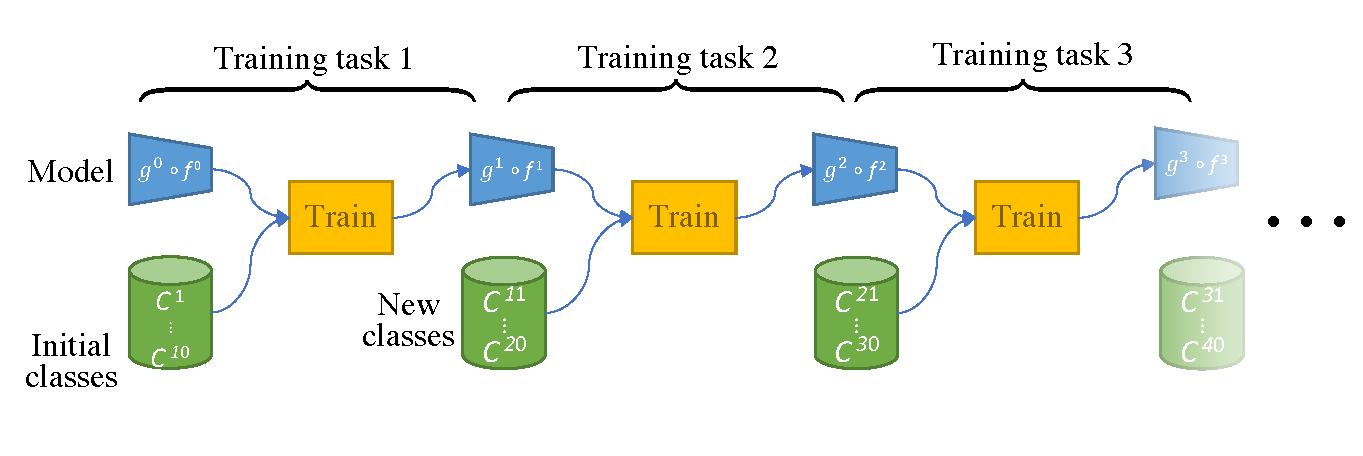
\includegraphics[width=1.0\linewidth]{images/related/protocol}
      \end{center}
      \caption{\textbf{Training protocol for incremental learning}. At each training task we learn a
            new set of classes, and the model must retain knowledge about \textit{all} classes. The
            model is allowed a \textit{limited} memory of samples of old classes.}
      \label{fig:related_protocol}
\end{figure}

\paragraph{Class-Incremental Example} More concretely, a common benchmark in \acf{CIL} is learning
the image classification CIFAR100 dataset \citep{krizhevskycifar100}, made of 100 classes, in
multiple steps, each made of several new classes. During the first step $t=1$, the model $g^1 \circ
      f^1$ learns the first 10 classes $\mcC^{t=1}$. During the second step $t=2$, the model $g^2 \circ
      f^2$ is initialized from the learned parameters of the previous model $g^1 \circ f^1$ and learns the
next 10 classes $\mcC^{t=2}$., and so on, until all 100 classes are learned at the last step $t=T$.
After each step, we evaluate the model on the testing data of all seen classes $\mcC^{1:t}$.
\autoref{fig:related_protocol} illustrates such continual protocol, and
\autoref{fig:related_forgetting} depicts the continual performance of a both trained from scratch on
all data for each task and a continual model finetuned only on new data. The continual model
over-predicts new classes \citep{davidson2020masteryincremental} and has a low overall accuracy due
to a forgetting of old classes. This clearly illustrates how important is the catastrophic
forgetting. While in this thesis we mainly tackle \acf{CIL} benchmarks, we describe other continual
benchmarks in detail in the appendix (\autoref{sec:related_variation}).

\begin{figure}[tb]
      \begin{center}
            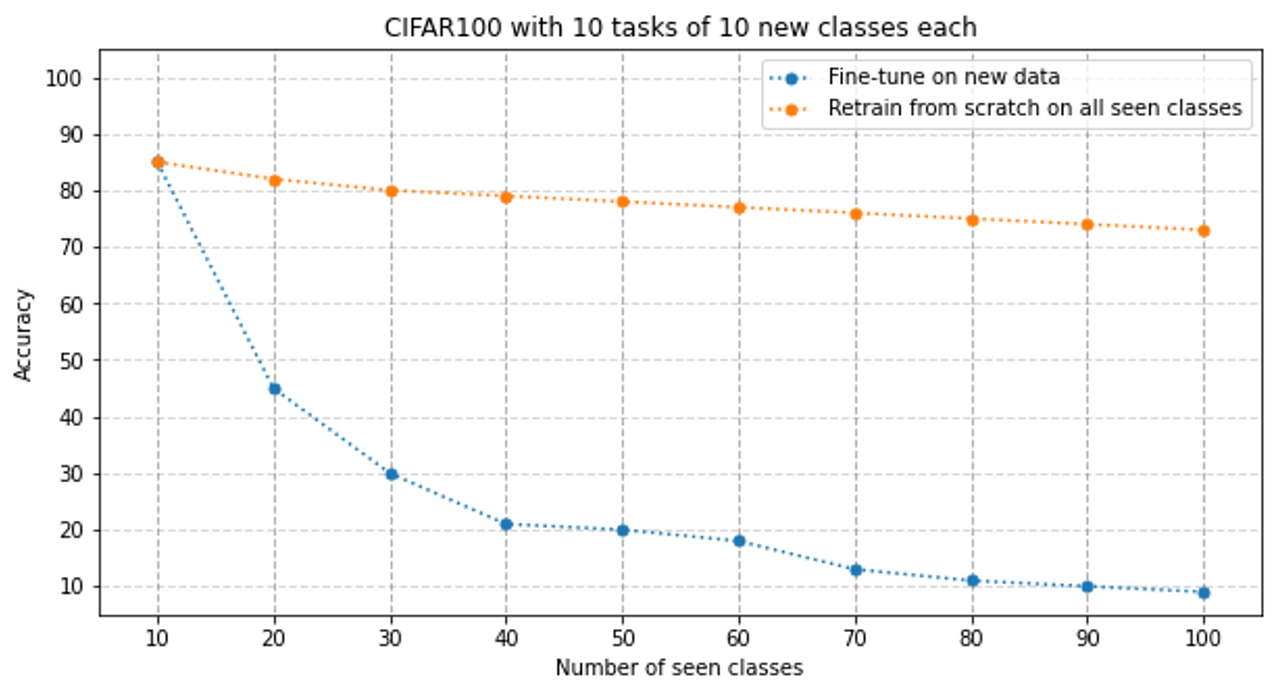
\includegraphics[width=0.8\linewidth]{images/related/catastrophic_forgetting.png}
      \end{center}
      \caption{\textbf{Illustration of the forgetting in Class-Incremental Learning}.
            \textcolor{orange}{orange} line displays the accuracy of a model which is re-trained from
            scratch at each step on all previous training data $\mcC^{1:t}$. This model, usually called
            Joint, is considered as a reasonable upper bound. On the other hand, the
            \textcolor{blue}{blue} line is a model finetuned solely on new classes $\mcC^{t}$ without
            access to previous classes $\mcC^{1:t-1}$. The gap between both models illustrates the
            catastrophic forgetting.}
      \label{fig:related_forgetting}
\end{figure}

\paragraph{Single-Head \vs Multi-Heads} are the two main evaluation settings in Continual Learning
\citep{chaudhry2018riemannien_walk}. In the former setting, a model has to classify samples among
all seen classes $\mcC^{1:t}$, that could have been learned from any of the seen steps. On the other
hand, in a multi-heads setting, a model knows at test-time the step/task identifier $i$ of the
samples. Thus, it only has to classify among the limited number of classes brought by a step
($\mcC^i$). Multi-Heads evaluation is closely related to multi-tasks learning. During this thesis,
we focus on the Single-Head evaluation because it is more realistic as it is rarely possible to know
from which step a sample comes from in a real-life setting. This setting is also more challenging
because a unique classifier must discriminate among all tasks' classes instead of having a different
classifier per task \citep{lesort2019regulshortcomings}.


%\subsection{Metrics for Continual Learning}
\label{sec:related_metrics}

\paragraph{Metrics} Multiple metrics exist in Continual Learning: the most common are the
\textbf{final accuracy} and \textbf{average incremental accuracy}. The former measures the
performance of the model on all tasks at the last step, the latter measures the average of
performance on all seen tasks after each new task learned \citep{rebuffi2017icarl}. Practically,
given $A_{i,t}$ the accuracy of the $i^{th}$ task after learning the $t^{th}$ task, the final
accuracy is (assuming balanced tasks):
%
\begin{equation}
      \text{Acc}_F = \frac{1}{T} \sum_{i=1}^T A_{i,T}\,,
      \label{eq:related_final_acc}
\end{equation}
%
and the average incremental accuracy:
%
\begin{equation}
      \text{Acc}_a = \frac{1}{T} \sum_{t=1}^T \frac{1}{t}  \sum_{i=1}^t A_{i,t}\,.
      \label{eq:related_avg_acc}
\end{equation}
%
Average incremental accuracy is somewhat more important than simply the final accuracy: a continual
model should be good after every step because in a true continual setting, there is not a ``final
task''.

Other metrics exist \citep{diaz2018continualmetrics}, such as \textbf{forgetting}
\citep{chaudhry2018riemannien_walk} which records how much a model has lost performance-wise on a
task compared to the first time it has learned it. The interest of this metric is to be agnostic of
the absolute performance of the model used.

Finally, metrics such as \textbf{speed} (\ie the number of images processed per second) or used
\textbf{capacity} (\ie number of learned parameters) are important:
\citet{ramasesh2022scalecontinual} recently showed that the larger a model was the lower was the
forgetting.

\section{Methods to reduce forgetting}
\label{sec:related_methods}

Multiple approaches exist to reduce forgetting in Continual Learning. The major ones are
rehearsal of old data (\autoref{sec:related_rehearsal}), regularizations constraining the model's
behavior (\autoref{sec:related_regul}), and structural adaptations (\autoref{sec:related_structural}).

\subsection{Rehearsal Learning}
\label{sec:related_rehearsal}

The most efficient method to reduce forgetting is \textbf{rehearsal learning} where old samples will
be seen alongside the new samples. The amount of old samples stored is extremely limited, otherwise,
it would defeat the purpose of continual learning. \autoref{fig:related_protocol_rehearsal} illustrates how
rehearsal learning happens in Continual Learning. During the first step, a model is trained on all
available samples. Then, it stores a limited amount of those in a \textit{memory}. During the second
step, the model has access to new samples but also all samples stored in the memory. In
Class-Incremental, an equal amount of samples per class is stored in memory. There are
two major approaches to determine this amount: \citet{rebuffi2017icarl} propose to fully use a
memory of size $\mcM$ among all $\mcC$, while \citet{hou2019ucir} instead kept fixed the number of
samples stored per class to $\nicefrac{\mcM}{|\mcC^{1:T}|}$.

\begin{figure}[tb]
      \begin{center}
            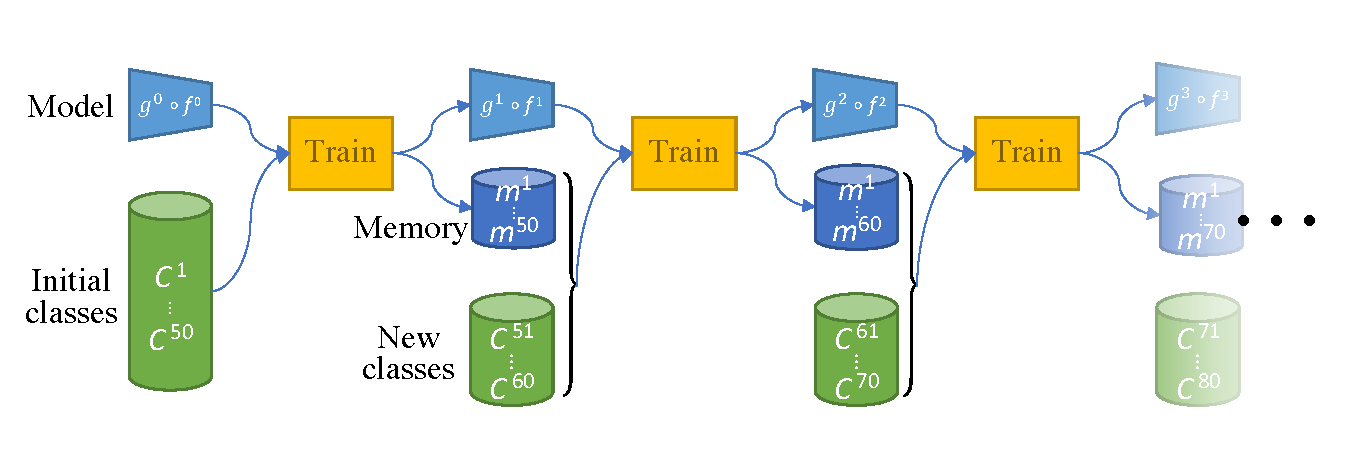
\includegraphics[width=1.0\linewidth]{images/related/rehearsal}
      \end{center}
      \caption{\textbf{Training with a rehearsal memory}. After each task a fraction of the
            data is stored in a memory to be used in the next task. Rehearsal learning is the most
            efficient method to reduce forgetting, but unfortunately the memory capacity is often
            extremely limited.}
      \label{fig:related_protocol_rehearsal}
\end{figure}

\paragraph{Herding} is the action of choosing which samples per class to store in the rehearsal
memory. The most naive herding method is to randomly sample images. Despite its simplicity, it is
quite competitive with more complex method \citep{castro2018end_to_end_inc_learn}, echoing similar
results in \ac{AL} \citep{gal2017activelearning}. Other herding methods include fetching samples
close to the class mean in the feature space \citep{castro2018end_to_end_inc_learn} or close to an
incremental barycenter \citep{rebuffi2017icarl}.

\paragraph{Sampling} is an important but yet fewly investigated topic in Continual Learning. Most
models mix all memory samples with new samples without any under- or over-sampling.
\citet{castro2018end_to_end_inc_learn} propose to finetune for a few epochs, after training on a new
step, on a balanced set of old and new classes samples. \citet{chaudhry2019tinyepisodicmemories}
oversample tiny memory with as low as one sample per class, and show, in the context of Online
Learning where models learn in only one epoch, that continual models still do not overfit. In the
same context, \citet{aljundi2019maximallyinterfered} propose to over-sample the memory examples with
the highest losses. In an imbalanced situation for Continual Learning, over- and under-sampling can be
applied depending on the number of samples per class \citep{kim2020imbalancedcontinual}.

\paragraph{Efficient Storing} is important for rehearsal learning: a bigger rehearsal memory leads
invariably to less forgetting \citep{hou2019ucir}. Thus, multiple works consider how to store more
rehearsal samples given the same memory size: \citet{hayes2020remind} compress intermediate features
of memory samples with a lossless compression algorithm.
\citet{iscen2020incrementalfeatureadaptation} also store features but modify them through the
training to handle the inherent internal covariate drift.

\paragraph{Pseudo-rehearsal} does not need to store samples but instead generates pseudo-samples for
rehearsal \citep{lesort2019generative}. The generation can be done with auto-encoders from
intermediate features \citep{kemker2018fearnet,ayub2021eec} or use \ac{GAN}
\citep{shin2017deep_generative_replay}. Unfortunately, those methods have several drawbacks: they
struggle to scale to large images, the generator size may be superior to a classic rehearsal memory
size which would defeat the goal of using less storage, and finally, the generator may itself suffer
from catastrophic forgetting \citep{zhai2019lifelonggan}. \citet{liu2020mnemonics} propose instead a
method halfway between rehearsal and pseudo-rehearsal: the authors randomly sample real images, and
then during continual training, slightly modify them via bi-level optimization
\citep{wang2018datasetdistillation} to minimize forgetting.


\subsection{Regularization-based Approaches}
\label{sec:related_regul}


\begin{figure}[tb]
      \begin{center}
            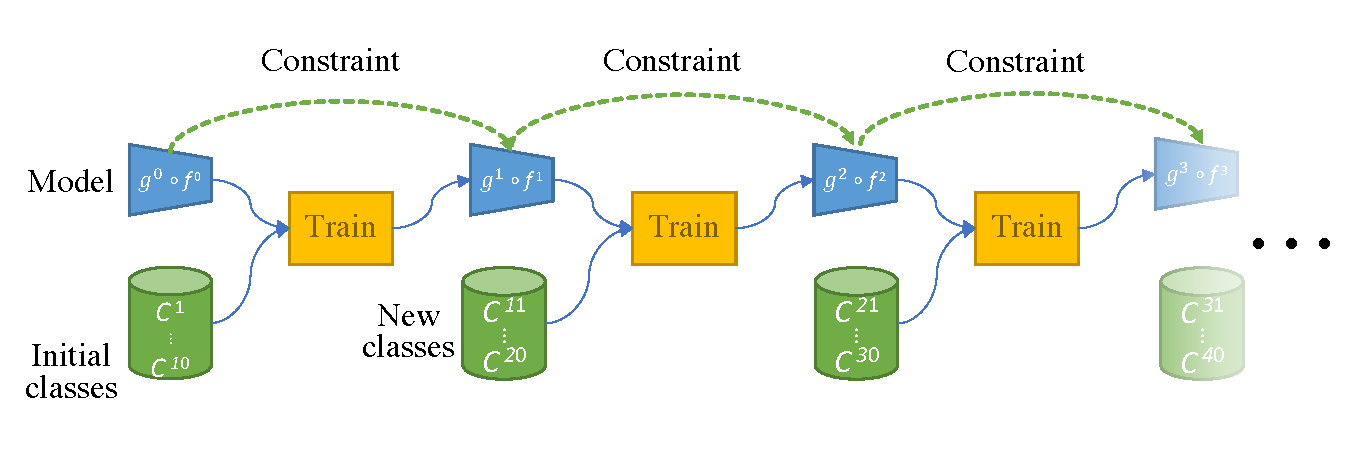
\includegraphics[width=1.0\linewidth]{images/related/constraints}
      \end{center}
      \caption{\textbf{Constraining the new model based on the old model}. During each task, after
            the first one, the new model is constrained to be similar to the old model in order to reduce
            forgetting.}
      \label{fig:related_protocol_constraints}
\end{figure}

A common and efficient way to reduce forgetting is to minimize the difference in behavior between
the old and new models as illustrated in \autoref{fig:related_protocol_constraints}. These constraints can be
expressed through various forms and are described below.

\subsubsection{Weight-based constraints}
\label{sec:related_regul_weight}


The most straightforward way to avoid completely forgetting is that the old and new models stay
identical. While the model would be \textit{rigid} (no forgetting), it is also not \textit{plastic}
(changing a lot) at all, and thus cannot learn any new tasks. Thus, a line of research proposed to
constrain only a portion of the neurons:
%
\begin{equation}
      \mcL(\theta^t, \theta^{t-1}) = \mcL_t(\theta^t) + \lambda \sum_i \Omega_i^{t-1} (\theta^t_i - \theta_i^{t-1})^2\,,
      \label{eq:related_weight_constraint}
\end{equation}
%
where $\mcL_t(\theta)$ is the loss at the current task $t$ (\eg the cross-entropy), $\theta_i^t$
and $\theta_i^{t-1}$ respectively the $i^\text{th}$ neuron of the current and previous model, and
$\Omega_i^{t-1}$ a neuron-wise importance factor. The intuition is that important neuron for the
previous task $t-1$ should not change, while the others can be adapted to fit the new task $t$.

\citet{kirkpatrick2017ewc}, followed by \citet{zenke2017synaptic_intelligence} and
\citet{chaudhry2018riemannien_walk} propose to use the diagonal Fisher information matrix as
importance factors. The motivation behind was that the posterior $p(\theta^{t-1} | \mcD^{t-1})$ must
contain the information about which parameters are important to the previous dataset $\mcD^{t-1}$.
This posterior can be approximated by a Gaussian distribution whose diagonal precision is given by
diagonal Fisher information matrix. A higher value means a more important neuron for the previous
task, and thus the constraint should be increased proportionally. Thus, a lower value, for a less
important neuron, means that it can change drastically, which would facilitate learning new data.
This strikes a balance between rigidity (not changing and thus not forgetting), and plasticity
(changing, and thus learning new concepts). Note that \citet{aljundi2018MemoryAwareSynapses} instead
use the sensitivity of the model when small perturbations are added to the neurons to measure their
importance.

However, it is worth remarking that weight-based constraints are usually limited to the multi-heads
setting where a task identifier is available at test time. \citet{lesort2019regulshortcomings} show
that in the single-head setting, they struggle to reduce forgetting and are significantly
outperformed by the simple (but somewhat memory costly) rehearsal learning.

\subsubsection{Gradient-Based methods}
\label{sec:related_regul_gradient}

\begin{figure}[tb]
      \begin{center}
            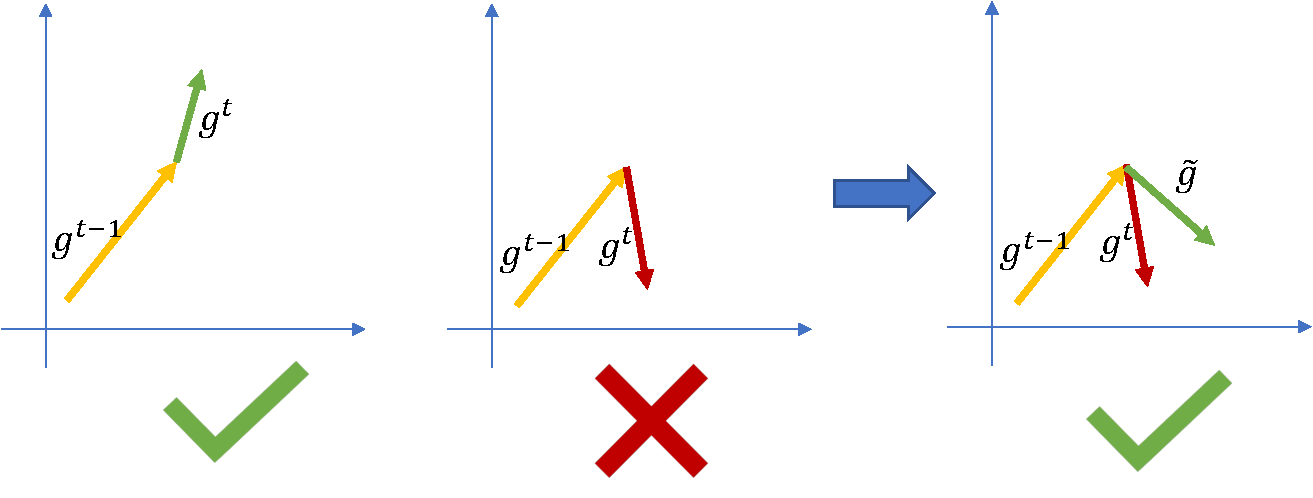
\includegraphics[width=1.0\linewidth]{images/related/gem.pdf}
      \end{center}
      \caption{\textbf{GEM's gradient constraint} forcing updates to be in the same direction as the
            gradient \wrt old samples. In (a) the new gradient $g^t$ is valid, while in (b) the new gradient
            violates the constraint of $\langle g^t,\, g_{t-1}\rangle \ge 0$. In (c), the invalid gradient
            $g^t$ is projected to the closest valid alternative $\tilde{g}$.}
      \label{fig:related_gem}
\end{figure}

\citet{lopezpaz2017gem} propose the GEM model that combines a constraint on the gradients and
rehearsal learning. The algorithm requires that the loss on a given stored sample must not increase
despite the model learning new classes. The authors, given a locality assumption, rewrite this
formulation as enforcing that the gradient of a new sample ($g$) to be in the same \textit{direction} as
the gradient of all stored old samples ($g_i \, \text{for all}\, i \in \mcM$):
%
\begin{equation}
      \langle g,\, g_i\rangle \ge 0,\, \text{for all}\, i \in \mcM\,,
\end{equation}
%
\noindent with $\mcM$ the rehearsal memory. If the constraint is violated, the new gradient $g$ is
projected to the closest in L2 norm gradient that satisfies the angle constraint by minimizing a
quadratic program. The constraint is illustrated in \autoref{fig:related_gem}. The drawback of this
method is the computational cost that can grow prohibitively when the memory is too large.
\citet{chaudhry2019AGEM} propose Averaged-GEM to speed up GEM: the authors do not constraint the
gradient of individual memory samples but only the average of all memory samples.
\citet{aljundi2019gradientselection} also improved GEM's speed by selecting only a subset of the
memory samples that maximize the feasible region.

Differently, but still constraining the gradients: \citet{farajtabar2020ogd}'s OGD forces the gradients of
task $t$ to be orthogonal to gradients of task $t-1$. They use the Gram-Schmidt procedure to
orthogonalize the new gradients, allowing updates for the new task that minimally interfere with the
performance of old tasks. \citet{saha2021gpm}'s GPM does likewise but uses instead a k-rank
approximation of the SVD of the representation matrix.


\subsubsection{Output-based constraints regularizations}
\label{sec:related_regul_output}

Finally, the majority of Continual models that are benchmarked on large datasets (\eg ImageNet
\citep{deng2009imagenet}) use a combination of rehearsal
learning (\autoref{sec:related_rehearsal}) and constraints on the model's outputs.

LwF \citep{li2018lwf} and iCaRL \citep{rebuffi2017icarl} apply the \ac{KD}
\citep{hinton2015knowledge_distillation} on the model's probabilities. It usually consists in
minimizing the \ac{KL} between the probabilities of the old and new models:
%
\begin{equation}
      \mcL_\text{KD} = \operatorname{KL}(\operatorname{softmax}(\frac{\tilde{y}^{t-1}}{\tau}) \Vert \operatorname{softmax}(\frac{\tilde{y}^t}{\tau})\,,
\end{equation}
%
where $\tilde{y}^{t-1} = g^{t-1} (f^{t-1}(\vx))$ and $\tilde{y}^{t} = = g^{t} (f^{t}(\vx))$ are respectively the logits of the old and new model,
and $\tau$ a \textit{temperature} to soften the probabilities in order to give more importance to
the model confidence in other classes than the top one. These probabilities, nicknamed \textit{dark
      knowledge} by \citet{hinton2015knowledge_distillation}, contain additional information about the
model which are useful to distil. Note that in the context of Class-Incremental, the new model
predicts more classes than the old model, therefore, the \ac{KL} is only applied on the logits
common to both the old and the new models. The \ac{KD} is sometimes also defined as the binary
cross-entropy between the sigmoid-activated logits.

Constraining the probabilities is now so ubiquitous that most models include it in their base
losses. On the other hand, a few models considered constraining intermediate outputs. MK2D
\citep{peng2019m2kd} uses the \ac{KD} from both the final classifier and an auxiliary classifier
similarly to the Inception network \citep{szegedy2015inception}. \citet{hou2019ucir} maximize the
cosine similarity between the embeddings produced by the \ac{GAP}.
\citet{dhar2019learning_without_memorizing_gradcam} minimizes the L1 distance between the attention
maps produced by GradCam \citep{selvaraju2017gradcam}.

\subsection{Structural Strategies}
\label{sec:related_structural}

\begin{figure}[tb]
      \begin{center}
            {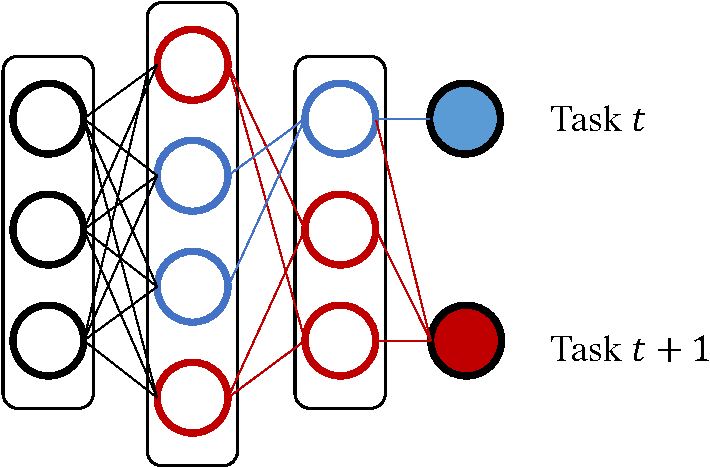
\includegraphics[width=0.5\linewidth]{images/related/subnetworks.pdf}}
      \end{center}
      \caption{\textbf{Task-specific subnetworks} that can be uncovered with a sparsity loss or
            learned masking. \textcolor{blue}{\textbf{Blue}} neurons are dedicated to
            the task $t$, \textcolor{red}{\textbf{red}} neurons to the following task
            $t+1$, and \textbf{black} neurons are shared among all tasks. At
            test-time, a task identifier of the sample is required to select the
            right subnetwork path.}
      \label{fig:related_subnetwork}
\end{figure}

Multiple works also propose to adopt dynamic strategies where the configuration of the neural
network evolves after each task. Critically, not only the number of neurons changes in the classifier $g^t$
(to incorporate new classes to predict), but the feature extractor $f^t$'s neurons count or organization
will also differ from its previous iteration $f^{t-1}$.


\paragraph{Subnetworks} The Lottery Ticket Hypothesis \citep{frankle2019lottery_ticket} states that
subnetworks made of a fraction of the neurons and connections of a larger network, can reach
excellent performance. Several Continual Learning models exploit that property by using a
subnetwork per task. Those subnetworks can be uncovered via genetic algorithms
\citep{fernando2017path_net}, via induced L1 sparsity \citep{golkar2019neural_pruning}, or even
learned masked \citet{serra2018hat,hung2019cpg}. Usually, these methods require a task identifier at
test-time in order to select the right subnetwork (see \textit{multi-heads} in
\autoref{sec:related_continual}). Later, \citet{wortsman2020supermasks} propose to infer the task
identifier by selecting the subnetwork with the lowest entropy. This subnetwork-based approach is
illustrated in \autoref{fig:related_subnetwork}.

\paragraph{Dynamically Expandable Networks} A neural network can also be expanded through its continual
training to accommodate the growing amount of tasks to solve. First, \citet{rusu2016progressive}
propose to have one network per task, where the $i^{\text{th}}$ network would depend both on the
input and all previous networks' intermediate features. Unfortunately, memory consumption is
quickly prohibitive with many tasks. Following works propose to only add blocks of parameters,
and only when deemed necessary \citep{veniat2021mntdp}. While these dynamic networks often require
an identifier at test-time to select the right subset of parameters, recently, DER
\citep{yan2021der} removed this need by learning a classifier upon the concatenated features of all tasks:
Their dynamic expansion of the representation adds a new feature extractor per task. All
extractors' embeddings would then be concatenated and fed to a unified classifier, discarding the
need for a task identifier at test-time. To limit an explosion in the number of parameters, they
aggressively prune each model after each task using the HAT \citep{serra2018hat} procedure.
Unfortunately, the pruning is hyperparameter sensitive. Therefore, hyperparameters are tuned
differently on each experiment: for example, learning a dataset in 10 steps or in 50 steps use
different hyperparameters. While being impracticable, it is also unrealistic because the number of
classes is not known in advance in a true continual situation. Simple-DER \citep{li2021preserve}
also uses multiple extractors, but its pruning method doesn't need any hyperparameters; the negative
counterpart is that Simple-DER controls less the parameter growth.

\paragraph{Task Conditioning} Rather than adding many new parameters, it is also possible to only
add a few parameters that will adapt the existing network behavior for a task.
\citet{rebuffi2017visualadapters} propose to add a different residual per task: given a task
identifier, the associated residual is used, and the features are modulated to best fit the given
task. Instead of adapting the features, \citet{wen2020batchensemble} and \citet{sun2019metatransfer}
propose to share most of the weights across tasks, but have task-specific weights that directly
modify the shared weights.

\paragraph{Mixture-of-Experts} Mixture of experts \citep{masoudnia2014mixture} have also been
proposed, where multiple experts combine their decision. \citet{aljundi2017experts} learn a gating
system to use the right task-specific expert. \citet{collier2020routingnetwork} stress the importance
on sharing experts when tasks are similar.
%\citet{yan2021der} and \citet{li2021preserve} proposed
%to have a \ac{ConvNet} per task and to concatenate their output embeddings to be fed to a single
%classifier. To avoid parameters explosion, they aggressively prune each \ac{ConvNet}.

\paragraph{Classifier Correction} Forgetting happens in both the feature extractor and the
classifier. Previously described rehearsal and regularization methods try to reduce it in both
places. On the other hand, multiple works focus solely on the classifier. They remark that in
\acf{CIL}, the classifier is miscalibrated \citep{guo2017miscalibration} where the model
over-predicts new classes to the detriment of old classes. \citet{belouadah2019il2m} compensate the
bias towards new classes by rectifying predictions of past classes using their recorded accuracies
and confidences. \citet{wu2019bias_correction} learn a linear model on validation data to recalibrate
the logits of the new classes. \citet{zhao2020weightalignement} normalizes the norm of the classifier
weights associated with new classes so that their average norm becomes the same as that for old
classes. \citet{hou2019ucir}, aims for a similar result by replacing the dot product in the
classifier with the cosine similarity, resulting in unit norm classifier weights.

\section{Positioning}

Continual Learning encompasses very different benchmarks and methods. In this PhD thesis, we tackle
multiple types of continual drift using different approaches. All the proposed strategies consider
the intermediary features of a neural network to reduce catastrophic forgetting. We summarize
below the three main chapters:

\paragraph{Feature-based Regularizations} First in \autoref{chapter:regularization}, we consider
\acf{CIL} scenarios with a prior drift where new classes are continually added. In this setting, our
approach consists in rehearsal learning (\autoref{sec:related_rehearsal}) and output-based
regularizations (\autoref{sec:related_regul_output}). Previous works reduced forgetting by
constraining either the final probabilities of the classifier \citep{li2018lwf} or the ultimate
embedding of the feature extractor \citep{hou2019ucir,dhar2019learning_without_memorizing_gradcam}.
In a first section (\autoref{sec:podnet}), we propose instead a regularization applied on several
intermediary levels of the features extractor. Moreover, few considerations have been made on how
the regularization loss makes the model more rigid, leading to less forgetting on old classes but
also impacting negatively the learning of new classes. Instead, we carefully define a regularization
loss, through pooling, balance effectively the performance of old and new classes. In a second
section (\autoref{sec:ghost}), we consider if the forgetting could be avoided preemptively.
\citet{aljundi2019selfless} consider allocating extra capacity implicitly in the learned feature
space for future classes using an unsupervised sparsity loss. Differently, we choose to draw from
weak metadata of the future unseen classes \citep{hanrebuffi2020autodiscovering} to estimate their
representation and thus explicitly allocate capacity, reducing forgetting before it even happens.

\paragraph{Continual Semantic Segmentation} Second, in \autoref{chapter:segmentation}, we tackle
\acf{CSS}. In this benchmark, defined recently by \citet{cermelli2020modelingthebackground}, images
have a label per pixel, and only the current classes are labelized. Thus, both the prior and concept
drifts happen where new classes are added but also the signification of a pixel can change through
time. In this setting, all previous works only considered regularizations
(\autoref{sec:related_regul_output}) based on the final probabilities
\citep{michieli2019ilt,cermelli2020modelingthebackground}. Instead, we expand from our previous
chapter to consider the multi-scale intermediary features. Moreover, no work directly tackled the
partial labelization of the images \citep{cermelli2020modelingthebackground}. We propose for this
challenge an uncertainty-based pseudo-labeling \citep{saporta2020esl}, and a new rehearsal method
(\autoref{sec:related_rehearsal}), optimized for segmentation.

\paragraph{Dynamic Transformers} In this third and last chapter (\autoref{chapter:dynamic}), we only
aim to solve the prior drift but using a method radically different from previous chapters: dynamic
networks (\autoref{sec:related_structural}). Previous dynamic networks usually expand their capacity
by a large margin during the continual training to handle the growing amount of tasks to learn
\citep{yan2021der}. To avoid a parameter count unbounded growth, the models are usually pruned
aggressively. The main drawback of these methods is that the pruning can still result in models too
large and often need careful finetuning of hyperparameters. We propose in this chapter, a dynamic
expansion based on the transformer architecture with almost no memory overhead contrary to
concurrent works, that conditions \citep{perez2018film} the intermediary features.
